\chapter*{POMCP}
\setcounter{page}{1}
\label{sec:pomcp}

% explain: 
% - Planning versus learning
% - Curse of dimensionality and how POMCP breaks it with Monte-Carlo sampling
% - Define state space dimensinality of Torcs problem
% - Belief and blief update
% - unweighted particle filter
% Stages of the simulation

\section*{Algorithm}

\begin{figure}[h]
    \centering
    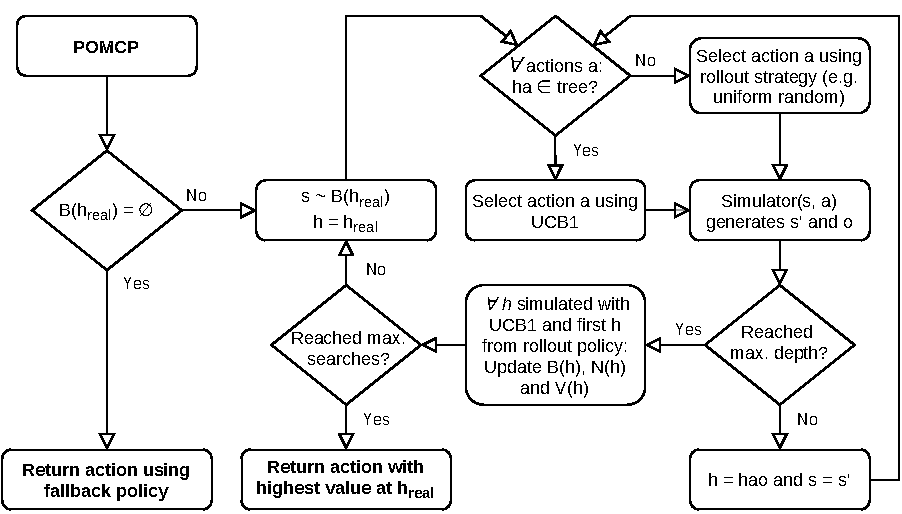
\includegraphics[width=\textwidth]{figures/POMCP.pdf}
\end{figure}

\Gls{pomcp} constructs a search tree with nodes representing histories $h$ of actions and observations. At each node, $N(h)$ stores the number of times the represented history $h$ has been encountered, $V(h)$ is the node's value that is approximated by the average return of simulations starting at history $h$, and $B(h)$ represents the node's belief over the real environment's state. $B(h)$ is a collection of potential states where the likelihood of each state is given by the relative number of times it is included in the collection.

If the belief at the node representing $h_{real}$ is empty, an initial state distribution $I$ is used to sample a start state $s$ for the search. Otherwise, $B(h_{real})$ is utilized. The search tree is then searched in two stages. First, in the case that the search tree already contains child nodes for all actions at the current history, UCB1 is used for the action selection. Exploration is achieved by increasing the value of rarely-tried actions by an exploration bonus. Second, when the tree is missing a node for a potential action at the current history, a rollout policy is used to select actions. In the most simple case, this means choosing uniformly random over the action space. In either case, the selected action is executed on the start state $s$, leading to a successive state $s'$, observation $o$, and reward $r$. The process is repeated with resulting successive states until a maximum depth of the tree is reached. Afterwards, the beliefs, counts, and values are updated at all nodes for the histories resulting from the UCB1 action selection, and the node for the first history resulting from the rollout policy. The belief is updated by adding the successive states $s'$ from the simulator to the collections $B(ho)$ in the nodes. If the maximum planning time has not yet been reached, another start state is sampled and the whole process repeats. When the time runs out, the action $a_{best}$ with the highest value at the current history $h_{real}$ is returned. After this action is executed in the real environment, with an observation $o_{last}$ the tree can be pruned. Only the nodes from history $h_{real}a_{best}o_{last}$ onward stay relevant as all other histories are rendered impossible.
